\section{논문 요약}{\label{sec:review}}

\subsection{Multi-modal fusion transformer for end-to-end autonomous driving}{\label{subsec:Transfuser}}
\begin{figure}[htp]
    \centering
    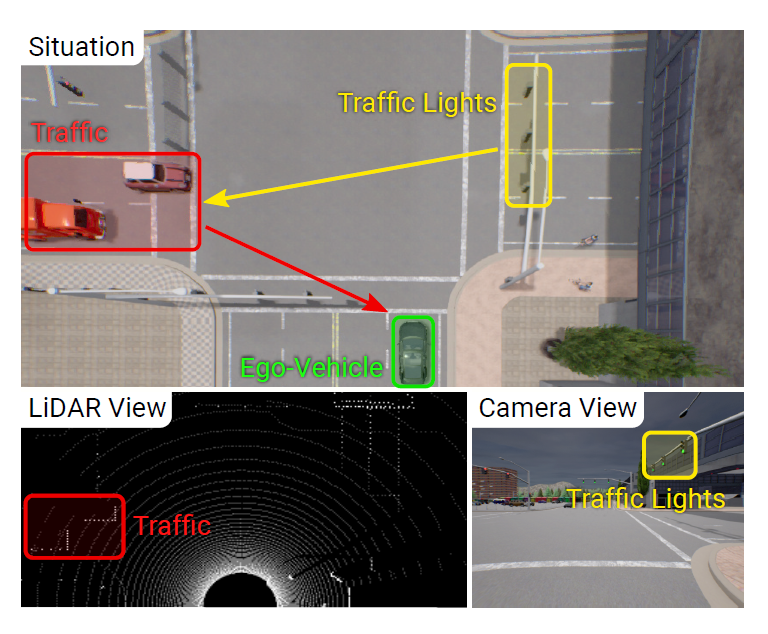
\includegraphics[width=0.8\textwidth]{figures/Transfuser_case.png}
    \caption{논문에서 해결하려는 문제 상황}
    \label{fig:tf_case}
\end{figure}
이 논문은 \autoref{fig:tf_case} 의 상황처럼
라이다(LiDAR : Light Detection And Ranging) 센서로 얻을 수 있는 주변의 차량의 위치에 따른 교통정보와
카메라로 얻을 수 있는 신호기에 따른 교통정보가 다른 경우,
두 센서로부터 얻을 수 있는 정보를 결합하여 차량의 주행을 제어하는 것을 목적으로 한다.
\begin{figure}[htp]
    \centering
    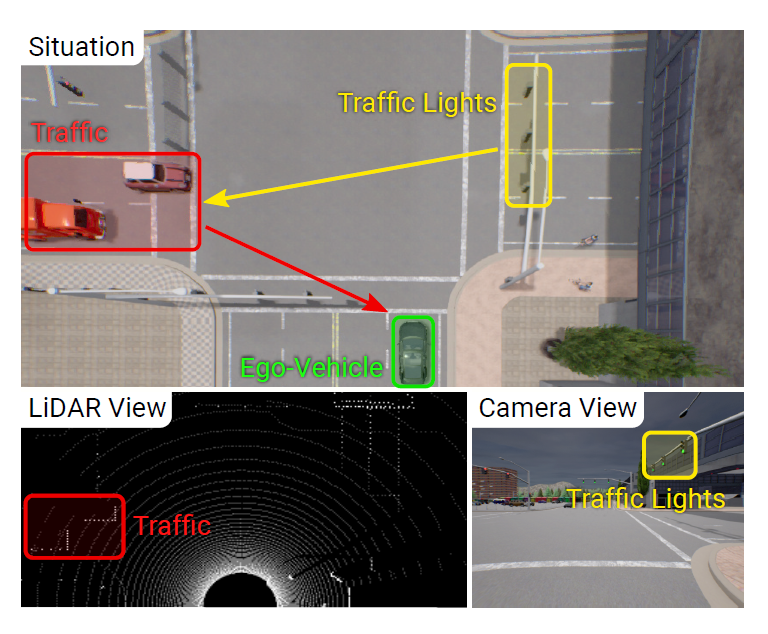
\includegraphics[width=\textwidth]{figures/Transfuser.png}
    \caption{Transfuser 구조}
    \label{fig:tf}
\end{figure}
\autoref{fig:tf}는 Transfuser의 구조를 보여준다.
두 센서의 출력으로부터 Resnet 구조\cite{Resnet}를 이용하여 정보를 추출하는 과정에서,
각 layer의 출력단으로부터 추출된 정보를 Transformer\cite{Transformer}를 이용하여 결합하는 것을 확인할 수 있다.

\subsubsection{method}{\label{subsubsec:tf_method}}
% 목적, 입력, 전처리, 출력, 학습, 평가
\paragraph*{목적} 논문에서 제시한 목표는 시내 도로 주행에서의 point-to-point navigation이다.
point-to-point navigation은 차량이 목표지점까지
waypoint를 따라
교통법규를 지키면서
다른 차량과의 상호작용을 하며
완주하는 것을 의미한다.
이를 달성하기 위한 방법으로 강화학습 기법 중 하나인 Imitation Learning을 채용하였다.
Imitation Learning은 전문가가 직접 주행한 데이터를 따라하도록 agent의 policy를 학습하는 것을 의미한다.

\paragraph*{입출력} 자율주행 오픈소스 시뮬레이터 CARLA\cite{CARLA}에 있는 urban 가상환경에서 수집한 데이터를 입출력으로 사용하였다.
\textbf{입력}은 두 가지로, 카메라와 라이다 센서의 출력이다.
카메라로부터 얻은 영상의 왜곡을 줄이기 위해 이미지 입력의 중앙을 잘라내어 $256 \times 256 \times 3$  크기로 사용했다.
LiDAR 센서의 출력 또한 주변부분의 정보를 기반으로 $256 \times 256 \times 2$ 사이즈로 잘라내어 사용하였다.
채널의 한쪽은 지면 위, 한쪽은 지면 아래를 의미한다.
\textbf{출력}은 PID controller로 차량을 제어하기 위해 4개의 waypoint $\{w_t = (x_t, y_t)\}_{t=1}^T$ 로 설정했다.

\paragraph*{모델}
모델은 \autoref{fig:tf}에서 두 가지 부분으로 나눌 수 있다.
첫째는 Resnet과 Transformer를 이용하여 구성한 Multi-Modal Fusion Transformer(Transfuser)이고,
둘째는 MLP와 GRU로 구성된 Waypoint Prediction Network이다.
먼저 Transfuser의 동작을 살펴보자.
전반적인 동작은 \autoref{subsec:Transfuser} 의 표제 문단에서 작성하였으므로 Transformer의 적용 방법만을 확인한다.
Transformer로는 GPT 모델을 사용하였다.
\begin{itemize}\tightlist
    \item 라이다 입력과 영상 입력에 대해 컨볼루션과 풀링을 진행하여 채널 수를 늘리면서 특징을 추출한다.
    \item 특징의 크기를 average pooling을 통해 8x8 로 줄인다.
    \item 각 특성맵을 concat하여 16x8 크기의 특성맵을 만든다.
    \item velocity를 value로, 16x8 특징을 key와 query로 사용하여 self attention(dot product attention)을 적용한다.
    \item bilinear interpolation을 통하여 원본 영상의 크기로 확대한다.
    \item 이전 단의 특성맵과 attention을 통해 추출한 특성맵을 더하여 특성맵을 업데이트한다.
\end{itemize}
둘째로 Waypoint Prediction Network의 동작을 살펴보자.
\begin{itemize}\tightlist
    \item activation이 ReLU인 3-Layer Perceptron을 이용하여
    $1 \times 1 \times 512$ 크기의 특징을
    $1 \times 1 \times 64$ 크기의 특징으로 압축한다.
    \item 압축된 특징을 GRU에 입력하여 4개의 waypoint를 예측한다.
\end{itemize}

\subsubsection{result}
\begin{figure}[htp]
    \centering
    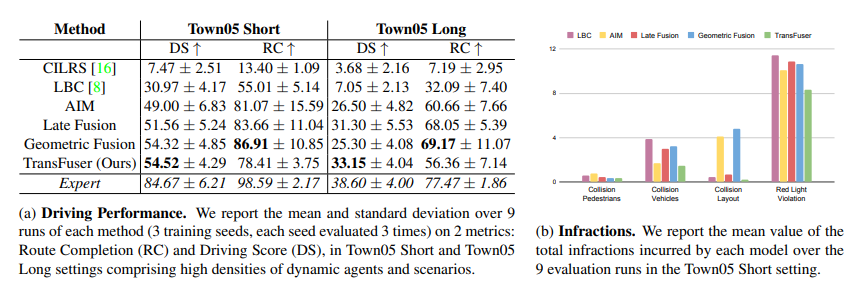
\includegraphics[width=0.8\linewidth]{figures/Transfuser_result.png}
    \caption{Transfuser 실험 결과}
    \label{fig:tf_res}
\end{figure}

\subsection{YOLOv7: Trainable bag-of-freebies sets new state-of-the-art for real-time object detectors}{\label{subsec:yolov7}}

asdf